%!TEX root=../template.tex


\subsection{Configuration}

We use gem5 simulator to simulate CPU, cache etc, use NVMain simulator simulate DRAM, NVM, hybrid memory for all experiment in the report, and evaluate power and timing with McPAT ~\cite{mcpat}. The gem5 simulator supports four different CPU models: AtomicSimple, TimingSimple, In-Order, and O3. The current default CPU mode for gem5 is AtomicSimple mode, which is not enable by default for NVMain when atomic CPU model is used, since this model is typically used for fast-forwarding and warmups. It is note that cycle accurate simulation is not possible using this CPU model. In our experiment O3 CPU mode is used when integrating NVMain with gem5, which is a pipelined, out-of-order CPU model.   



                              
The L1 cache parameters were kept constant for all experiments. The L2 cache is 256kB 8-way set associative. L3 cache is 1MB 16-way set associate. All caches in the baseline use a 64B line-size. The setting in shown in ~\Tbl{tbl:cacheset}. Throughout this paper, LRU denotes the traditional LRU policy which inserts all incoming lines in the MRU position. Unless stated otherwise, all caches use the LRU policy for replacement decisions and these cache size setting. 


\begin{table}[ht]
\centering
\caption{\small Baseline System Configuration.}
\begin{tabular}{|c|c|}
\hline 
L1 inst. cache                       & 32kB, 64B linesize, 4-way \\ \hline
L1 data cache                        & 32kB, 64B linesize, 4-way \\ \hline
L2 private cache                     & 256kB, 64B line size, 8-way  \\ \hline
L3 shared cache                      & 1M, 64B linesize, 16-way \\ \hline
\end{tabular}
\label{tbl:cacheset}
\end{table}




\subsection{Benchmark}
SPLASH-2 benchmark is used in our experiment applied for X86 ISA. SPLASH-2 benchmark suite [4] includes applications and kernels mostly in the area of high performance computing (HPC). It has been widely used to evaluate multiprocessors and their designs. We use input parameters from SPLASH-2 source codes.  We compile the source code with -pthread and -static flag, which enable the program to run in gem5 simulator without error. 


%\begin{figure}[ht]
\begin{figure}[t]
\centering
%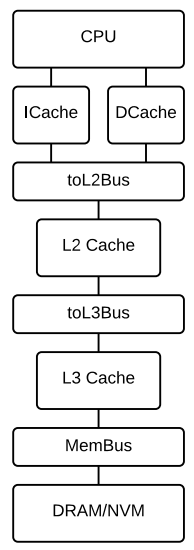
\includegraphics[width=\columnwidth]{figs/llc}
%\includegraphics[trim=0 0 0 0, clip, width=\columnwidth]{figs/browser-arch}
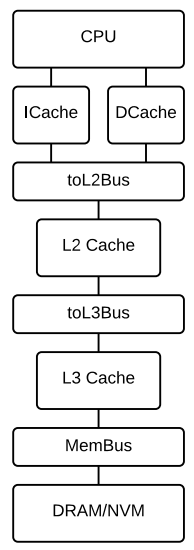
\includegraphics[scale=0.7]{figs/llc}
\caption{Simulation Architecture with L3 Cache.}
\label{fig:llc}
\end{figure}




\subsection{L3 Cache}
In the default gem5 simulator, it only integrate two level cache with L1 data/instruction cache and L2 data cache. However, this configuration is not practical in modern computer system which usually includes share level 3 cache to reserve more data and to reduce the average time to access data from main memory ~\cite{6835921}. In contrast to L1 and L2 cache, both of which tend to be private and dedicated to the needs of particular core. The new added share L3 cache will improve existing gem5 memory hierarchy. In the experiment, we build a shared L3 cache in gem5, it is connected to memory through Membus and connected to L2 cache through toL3Bus. L2 cache is connected to L1 cache through  toL2Bus, and L1 cache is connected to CPU and toL2Bus. The configuration is shown in ~\Fig{fig:llc}. There are several existing memory implementation in gem5 such as DDR3, LPDDR3 and  SimpleMemory in MemConfig.py file and its default value is DDR3. What's more, we integrate NVmain into gem5 to analyze non-volatile memory behavior such as PCM, STT-RAM and hybrid PCM with DRAM.  



\subsection{Cache Replacement Policy}
The traditional LRU replacement policy inserts all incoming lines in the MRU position. Inserting the line in the MRU position gives the line a chance to obtain a hit while it traverses all the way from the MRU position to the LRU position ~\cite{fan}. This is a good strategy for workloads whose working set is smaller than the available cache size or for workloads that have high temporal locality. To investigate impact of different cache replacement policy on the NVM architecture, we first turn to Non Most Recently Used cache policy (NMRU), which replace the least recently used cache block and insert new data in random cache block except the most recently used cache block. Similarly, we also look at the LRU Insertion Policy cache policy, which insert new data in LRU position instead of MRU position. Finally, we evaluate Random replacement cache policy.  In the experiment we used LRU policy as evaluation baseline, and change cache replacement policy to NMRU, LIP and Random Replacement policy under NVM environment ~\cite{Qureshi}. In gem5 simulator, the default cache replacement policy of all level cache is LRU, to further evaluate the impact of cache replacement policy on system, we use different combination of replacement policy in different level cache.     



\subsection{Hybrid Memory}
We built a hybrid memory system by integrating gem5 and NVMain, which uses a hardware-based page migrator to demonstrate the usefulness of advanced memory controllers and memory hooks. This simulated system uses a memory controller which employs a lookup table to find the destination of migrated pages and launch migration accordingly. This implementation uses a biased coin to decide whether to migrate a page or not for simplicity. Each time a request is issued, there is a small chance it will be migrated to another memory channel designated as “fast” memory. In theory, if a page is truly a “hot page”, it will eventually be migrated to fast memory. In this example, DRAM is used as fast memory and the remaining channels use NVM as slow memory. Migrations are done by using a single swap buffer. In the experiment, we set one channel to be DRAM and three channels to be NVM, STT-RAM and PCM are evaluated separately.   





\subsection{Clean Write Back Avoidance}
When dirty line is replaced in the cache, the data line is transferred to lower level memory hierarchy, this policy called write back. However, there is data line is not dirty but still write back to memory. We enable ruby 1-level cache coherence option and add additional debug option in gem5 to observe clean and dirty write-back counts. And we find that there is large number of clean write back to memory from cache, which will have negative impact on NVM architecture because of its high write latency and power. Thus, we modify corresponding gem5 source code to remove unnecessary clean write back based on MI\_example. The cache coherence is bottleneck in multi-core cpu architecture, so we need to find tradeoff between cache coherence and performance.   




